% Created 2024-04-21 Sun 21:34
% Intended LaTeX compiler: pdflatex
\documentclass[presentation]{beamer}
\usepackage[utf8]{inputenc}
\usepackage[T1]{fontenc}
\usepackage{graphicx}
\usepackage{longtable}
\usepackage{wrapfig}
\usepackage{rotating}
\usepackage[normalem]{ulem}
\usepackage{amsmath}
\usepackage{amssymb}
\usepackage{capt-of}
\usepackage{hyperref}
\mode<beamer>{\usetheme{Madrid}}
\definecolor{SUred}{rgb}{0.59375, 0, 0.17969} % SU red (primary)
\definecolor{SUblue}{rgb}{0, 0.17578, 0.38281} % SU blue (secondary)
\setbeamercolor{palette primary}{bg=SUred,fg=white}
\setbeamercolor{palette secondary}{bg=SUblue,fg=white}
\setbeamercolor{palette tertiary}{bg=SUblue,fg=white}
\setbeamercolor{palette quaternary}{bg=SUblue,fg=white}
\setbeamercolor{structure}{fg=SUblue} % itemize, enumerate, etc
\setbeamercolor{section in toc}{fg=SUblue} % TOC sections
% Override palette coloring with secondary
\setbeamercolor{subsection in head/foot}{bg=SUblue,fg=white}
\setbeamercolor{date in head/foot}{bg=SUblue,fg=white}
\institute[SU]{Shenandoah University}
\titlegraphic{
\includegraphics[width=0.5\textwidth]{\string~/Documents/suLogo/suLogo.pdf}}
\newcommand{\R}{\mathbb{R}}
\usetheme{default}
\author{Chase Mathison\thanks{cmathiso@su.edu}}
\date{22 April 2024}
\title{Power Series!}
\hypersetup{
 pdfauthor={Chase Mathison},
 pdftitle={Power Series!},
 pdfkeywords={},
 pdfsubject={},
 pdfcreator={Emacs 29.1 (Org mode 9.6.7)}, 
 pdflang={English}}
\begin{document}

\maketitle

\section{Announcements}
\label{sec:org62e40d1}
\begin{frame}[label={sec:orgeda6264}]{Announcements}
\begin{enumerate}
\item Homework.
\item Project.
\item Office hours canceled today.
\end{enumerate}
\end{frame}

\section{Lecture}
\label{sec:orgec690ff}
\begin{frame}[label={sec:org92dc4eb}]{Power Series}
\begin{definition}[Power Series]
A series of the form \[\sum_{n=0}^\infty c_n x^n = c_0 + c_1x+c_2x^2 +
\ldots\] is called a \alert{power series centered at 0}. A series of the form
\[\sum_{n=0}^\infty c_n (x-a)^n = c_0 + c_1 (x-a) + c_2 (x-a)^2+\ldots\] is
called a \uline{\hspace*{1in}}.
\end{definition}
\end{frame}

\begin{frame}[label={sec:org102c5f3}]{Example}
Which of the following are power series? What is the center of the power
series (if it's a power series)?

\begin{enumerate}
\item \(\sum_{n=0}^\infty \frac{x^n}{n!}\)

\item \(\sum_{n=2}^\infty \frac{(-1)^n}{n} (x-1)^n\)

\item \(\sum_{n=3}^\infty \frac{\sin(n x)}{n}\)
\end{enumerate}

\vspace{10in}   
\end{frame}

\begin{frame}[label={sec:orgd660b0e}]{A note on definitions}
\begin{block}{}
For consistency, we define \(0! = 1\) and \(x^0 = 1\), even when
\(x=0\).
\end{block}
\end{frame}

\begin{frame}[label={sec:org68a6746}]{Convergence of a power series}
It's always going to be the case that a power series converges at its
center \(x = a\). There are two other cases that could happen:

\begin{center}
\begin{center}
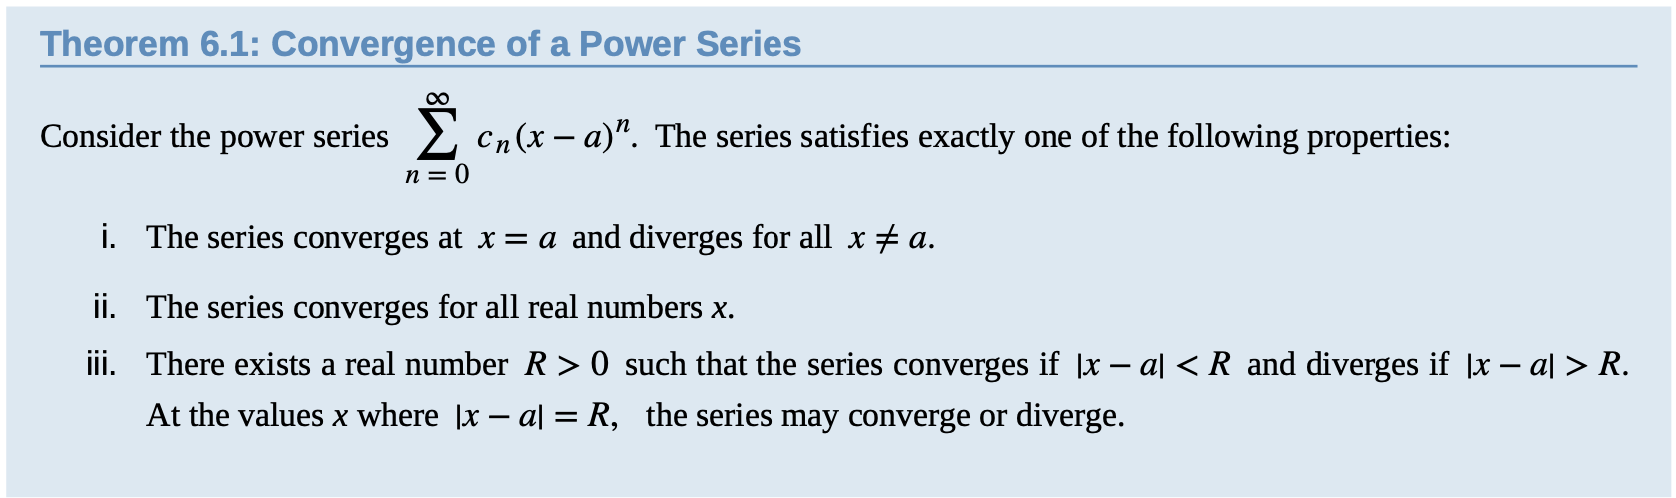
\includegraphics[width=.9\linewidth]{../img/convPowSer.png}
\end{center}\\[0pt]
\end{center}

\emph{Proof:}
\end{frame}


\begin{frame}[label={sec:org4fce166}]{Radius and interval of convergence}
The previous theorem leads to the following definitions:

\begin{center}
\begin{center}
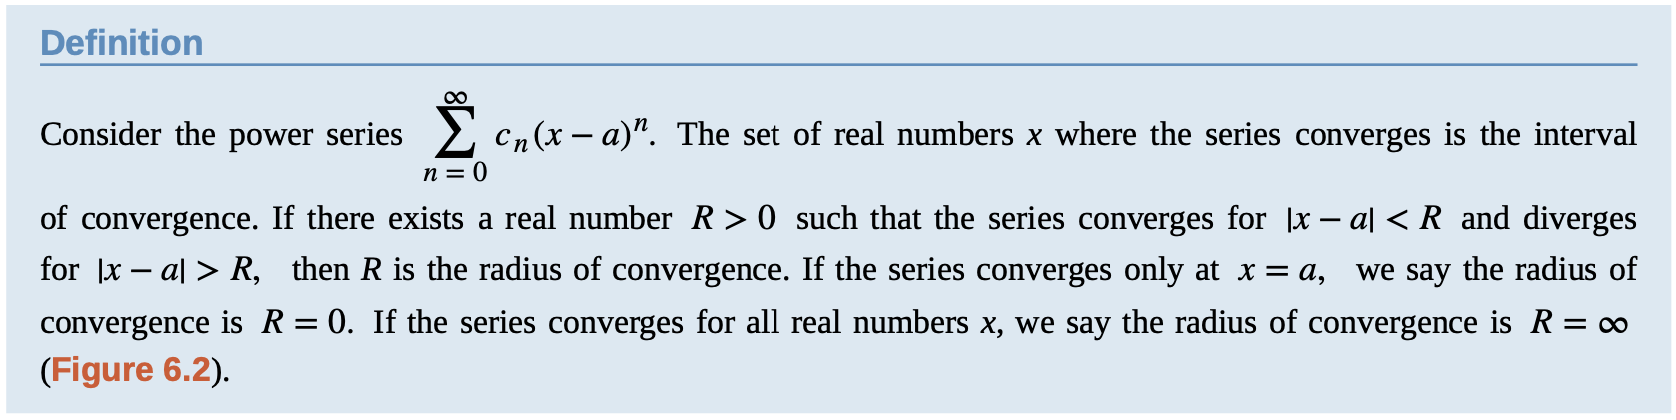
\includegraphics[width=.9\linewidth]{../img/rofConv.png}
\end{center}\\[0pt]
\end{center}

\vspace{10in}
\end{frame}
\begin{frame}[label={sec:orgd388929}]{Examples}
Find the radius of convergence and the interval of convergence
for the following power series (make sure to state the center of the
series).

\begin{enumerate}
\item \(\sum\limits_{n=0}^{\infty} \left( -1 \right)^n
      \frac{x^{n+1}}{n+1}\)

\item \(\sum\limits_{n=3}^{\infty} 2^n \left( x-3 \right)^n\)

\item \(\sum\limits_{n=1}^{\infty} \left( \frac{2x}{3} \right)^{2n}\)
\end{enumerate}

\vspace{10in}
\end{frame}

\begin{frame}[label={sec:orgd98cf65}]{Representing functions using power series}
We're one step closer to our ultimate goal, which is representing any
(reasonable) function using better and better polynomial
approximations. Let's look specifically at the function \[f(x) =
\frac{1}{1-x}.\]
\vspace{10in}
\end{frame}
\begin{frame}[label={sec:orgc1b9fb1}]{Representing functions using power series}
\end{frame}

\begin{frame}[label={sec:org784ef9b}]{Example}
Use the geometric series
\[\sum\limits_{n=0}^{\infty} ax^n = \frac{a}{1-x}\] to find what the
following power series converge to as functions. Make sure to find the radius
of convergence and the interval of convergence.


\begin{enumerate}
\item \(\sum\limits_{n=0}^{\infty} \left( -1 \right)^n x^n\)
\item \(\sum\limits_{n=1}^{\infty} \left( \frac{x}{3} \right)^{2n}\)
\end{enumerate}

\vspace{10in}
\end{frame}
\end{document}